\documentclass{standalone}
\usepackage{tikz}
\usepackage{ctex,siunitx}
\usepackage{tkz-euclide}
\usepackage{amsmath}
\usetikzlibrary{patterns, calc}
\usetikzlibrary {decorations.pathmorphing, decorations.pathreplacing, decorations.shapes,}
\begin{document}
\small
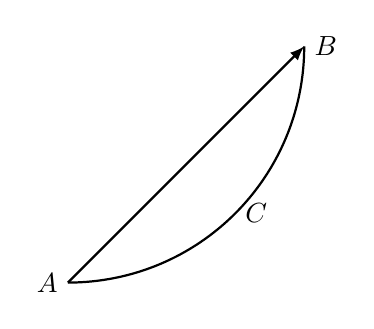
\begin{tikzpicture}[>=latex, thick]
  \draw [->](0,0)node[left]{$A$} --(3,3)node [right]{$B$} ;
  \draw (0,0) [bend left=-45]  to node [right]{$C$} (3,3);
\end{tikzpicture}
\end{document}